\documentclass[11pt]{article}

\usepackage{amsmath}
\usepackage{amssymb}
\usepackage[margin=0.68in]{geometry}
\usepackage{booktabs}
\usepackage{enumitem}
\usepackage{fancyhdr}
\usepackage{graphicx}
\usepackage[table]{xcolor}
\usepackage[hidelinks]{hyperref}
\usepackage{listings}
\usepackage{microtype}
\usepackage{tabularx}
\usepackage{tikz}
\usepackage{titlesec}
\usetikzlibrary{arrows.meta,decorations.pathmorphing,positioning}
\graphicspath{{docs/lessons/assets/}{../assets/}}

\definecolor{Ink}{gray}{0}
\definecolor{CodeGray}{gray}{0.96}
\definecolor{Soft}{gray}{0.90}
\hypersetup
{
    pdftitle={ADK Lesson 016: Matrix Keypad},
    pdfauthor={Kevin Shanahan},
    pdfsubject={Deterministic keypad scanning, debounce, and visible evidence},
    pdflang={en-US}
}
\pagestyle{fancy}
\fancyhf{}
\lhead{\textsc{ADK Lesson 016}}
\rhead{Matrix Keypad}
\cfoot{\thepage}
\setlength{\headheight}{14pt}
\setlength{\parindent}{0pt}
\setlength{\parskip}{5pt}
\setlist{nosep,leftmargin=1.45em}
\titleformat{\section}{\Large\bfseries\color{Ink}}{\thesection}{0.5em}{}
\titleformat{\subsection}{\large\bfseries\color{Ink}}{\thesubsection}{0.5em}{}
\lstdefinestyle{adkcpp}
{
    language=C++,
    backgroundcolor=\color{CodeGray},
    basicstyle=\ttfamily\small,
    keywordstyle=\color{Ink}\bfseries,
    commentstyle=\color{Ink},
    columns=fullflexible,
    keepspaces=true,
    showstringspaces=false,
    frame=single,
    rulecolor=\color{Ink},
    breaklines=true,
    tabsize=4
}
\newcommand{\checkbox}{\(\square\)}
\newcommand{\blank}[1]{\rule{#1}{0.4pt}}
\newcommand{\lessonbox}[1]{%
  \begin{center}
  \fcolorbox{Ink}{white}{\parbox{0.92\linewidth}{#1}}
  \end{center}}

\begin{document}

\begin{center}
  {\Huge\bfseries Make a 4x4 Keypad Talk}\\[4pt]
  {\Large Wire a few keys, win a light show, then finish the number pad}\\[8pt]
  \textit{Every correct key earns an immediate D13 celebration.}
\end{center}

\begin{tabularx}{\linewidth}{@{}>{\bfseries}l X >{\bfseries}l X@{}}
Lesson & 016 --- component & Time & 45--75 minutes\\
Prerequisites & Lessons 001--015 & Board & Arduino Mega 2560\\
Payoff & D13 patterns for every active key & Part & authorized 4x4 keypad\\
Safety & E1: USB-powered passive input circuit only\\
\end{tabularx}

\section{Mission}

Build one operator-input path:
\[
\text{4x4 keypad in 12-key mode}\rightarrow\texttt{MatrixKeypad}\rightarrow
\texttt{KeypadSnapshot}\rightarrow\text{D13 evidence}.
\]
\texttt{MatrixKeypad} owns and scans seven active pins. The real specimen is
an eight-wire 4x4 keypad: this first adventure uses all four rows and the
three number-pad columns while the identified A/B/C/D column is safely parked.
Its composed
\texttt{Keypad} interpreter debounces the 12-bit sample, maps one position to a
semantic key, and rejects chords until every key is released. Time enters only
through \texttt{update(now)}.

\lessonbox{\textbf{Boundary.} This lesson teaches input interpretation. It is
not a lock, credential system, or anti-ghosting keypad. A diode-less matrix can
produce ambiguous multi-key observations, so every chord is rejected.}

\subsection{Learning outcomes}

\begin{itemize}
  \item explain row selection and column pull-ups;
  \item separate electrical scanning from deterministic interpretation;
  \item predict debounce, press, release, and invalid-chord events;
  \item distinguish acquisition evidence from safe-state evidence;
  \item use RAII cleanup without exceptions, heap allocation, or blocking delay.
\end{itemize}

\section{Parts and safety}

\begin{tabularx}{\linewidth}{@{}l X@{}}
\toprule
Part & Requirement\\
\midrule
Arduino Mega 2560 & USB-powered board\\
4x4 membrane keypad & Passive switch matrix with identified eight-wire tail\\
Seven jumpers & D22 through D28; direct wiring, no breadboard needed\\
Insulating tape & Covers the unused A/B/C/D-column conductor by itself\\
Logic probe or oscilloscope & Optional TP-R0 observation; high-impedance input\\
\bottomrule
\end{tabularx}

Remove USB power before moving wires or attaching a probe. Identify the exact
eight-wire tail order with an unpowered continuity test; printed connector
order is not standardized. Label R0--R3 and C0--C3. Cover C3 by itself. No
keypad conductor connects directly to 5 V or GND.

\section{Authoritative wiring}

\begin{tabularx}{\linewidth}{@{}l l X@{}}
\toprule
Signal & Mega pin & Keypad contact\\
\midrule
Row0 / TP-R0 & D22 & row containing 1, 2, 3\\
Row1 & D23 & row containing 4, 5, 6\\
Row2 & D24 & row containing 7, 8, 9\\
Row3 & D25 & row containing *, 0, \#\\
Column0 & D26 & column containing 1, 4, 7, *\\
Column1 & D27 & column containing 2, 5, 8, 0\\
Column2 & D28 & column containing 3, 6, 9, \#\\
Column3 & parked & column containing A, B, C, D; insulated, no connection\\
Operator evidence & D13 & board LED; no external wire\\
\bottomrule
\end{tabularx}

This is direct wiring: the keypad does not plug into the breadboard. On the
Mega paired side header, D22/D23 form the first pair, then D24/D25, D26/D27,
and D28/D29. Follow that physical zig-zag and leave D29 empty.
During each scan, exactly one row becomes an output driven low. Active columns remain
inputs with internal pull-ups. A closed key pulls its column low. The selected
row immediately returns to input before the next row is selected.

\begin{center}
% ADK visual: pencil
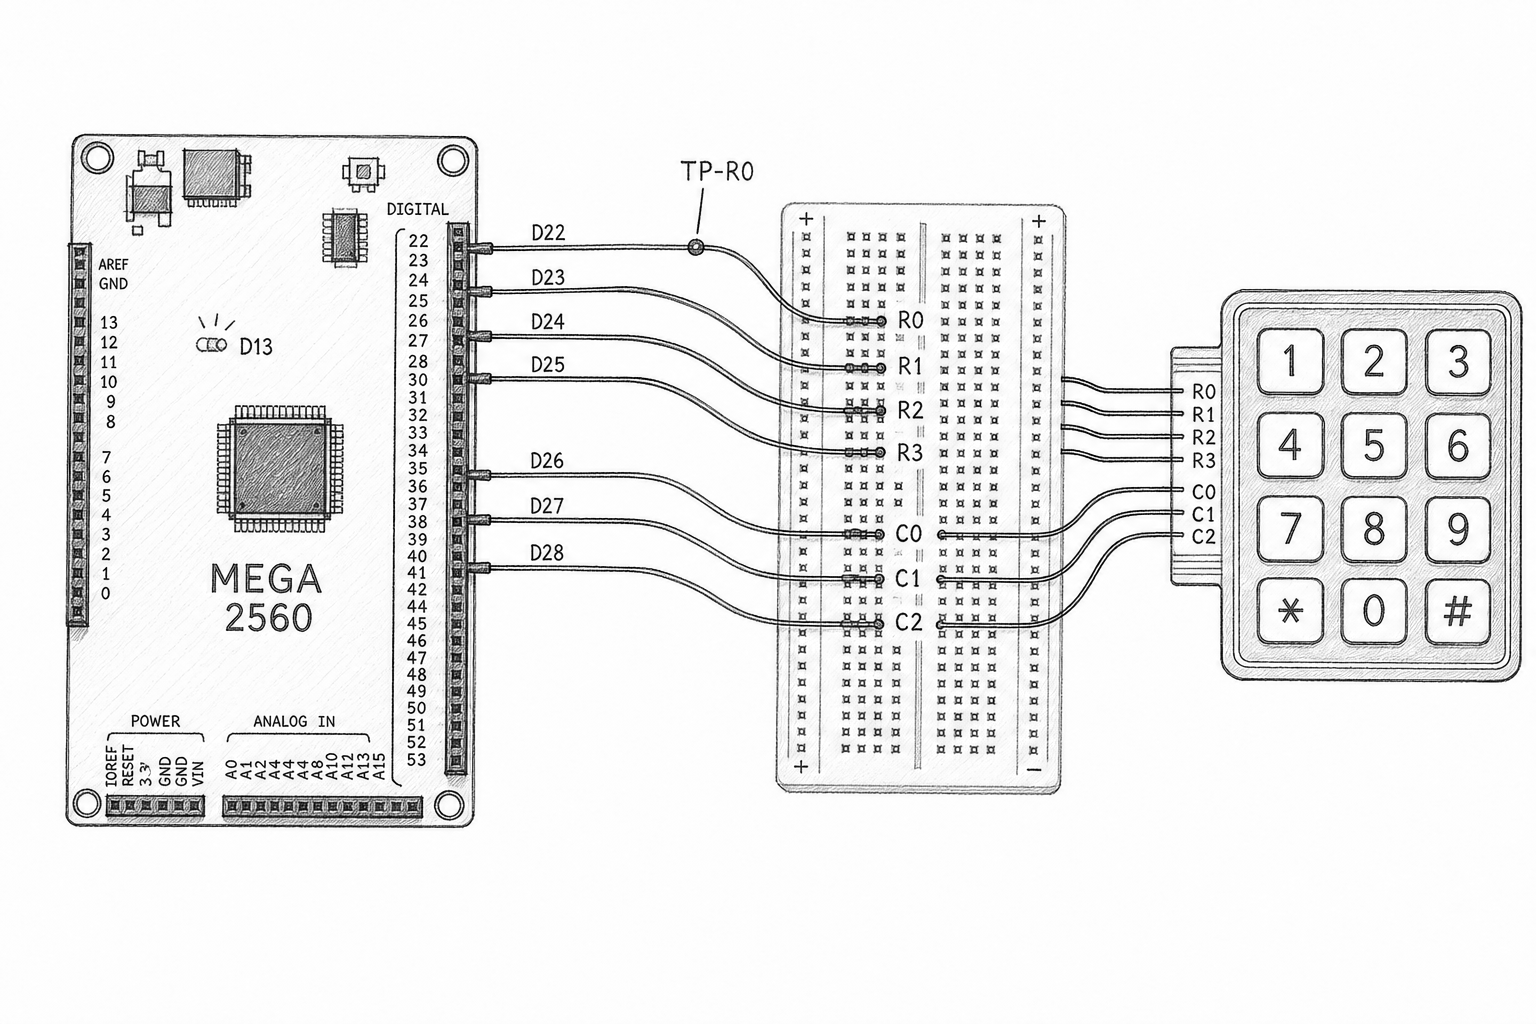
\includegraphics[width=0.96\linewidth]{016-matrix-keypad-pencil.png}

\small\textit{Alternative text: pencil orientation plate with a Mega on the
left and a 4x4 keypad on the right. The Mega side header shows its actual paired
D22/D23 through D28/D29 geometry. Seven labeled wires connect D22--D28 to
R0--R3 and C0--C2; C3, the A/B/C/D column, ends in its own taped parking tab.
There is no breadboard because every connection is direct.}
\end{center}

\section{Scan and interpretation}

\begin{center}
% ADK visual: pencil
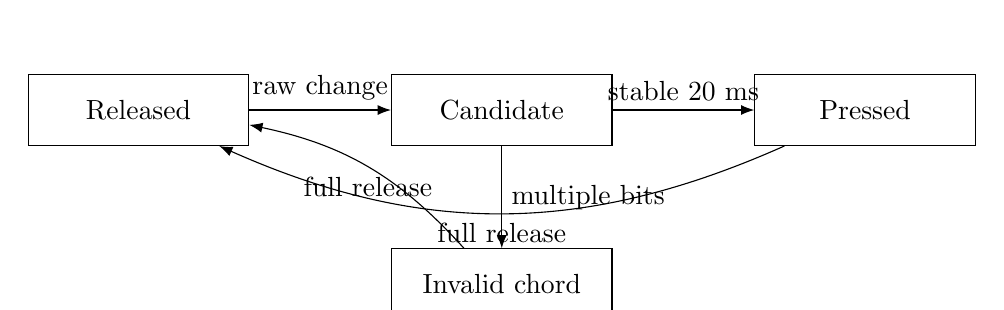
\begin{tikzpicture}[>=Latex,
    decorate,decoration={random steps,segment length=3pt,amplitude=0.18pt},
    state/.style={draw,minimum width=28mm,minimum height=9mm,fill=white}]
  \node[state] (released) {Released};
  \node[state,right=18mm of released] (candidate) {Candidate};
  \node[state,right=18mm of candidate] (accepted) {Pressed};
  \node[state,below=13mm of candidate] (invalid) {Invalid chord};
  \draw[->] (released)--node[above]{raw change}(candidate);
  \draw[->] (candidate)--node[above]{stable 20 ms}(accepted);
  \draw[->] (accepted) to[bend left=24] node[below]{full release}(released);
  \draw[->] (candidate)--node[right]{multiple bits}(invalid);
  \draw[->] (invalid) to[bend right=18] node[below]{full release}(released);
\end{tikzpicture}
\end{center}

A stable single bit produces one \texttt{pressEvent}. Holding the key produces
no repeats. A full stable release rearms the next press. A chord that collapses
to one key remains disarmed until complete release.

\begin{tabularx}{\linewidth}{@{}l l X@{}}
\toprule
Observation & D13 pattern & Interpretation\\
\midrule
Initialization & one short pulse & keypad and LED claims succeeded\\
Digit 1--9 & one to nine short pulses & accepted semantic digit\\
Digit 0 & ten short pulses & accepted zero, distinct from ready\\
* & one long pulse & accepted star\\
\# & two long pulses & accepted hash\\
Invalid chord & repeating two-short group & release every key before retry\\
Scan/update fault & repeating three-short group & stop relying on input\\
\bottomrule
\end{tabularx}

\section{Narrative code}

\begin{lstlisting}[style=adkcpp]
void loop ()
{
    if (!running)
    {
        return;
    }

    const adk::TimePoint      now         (millis ());
    const adk::KeypadSnapshot observation = observeKeypad       (now);
    const OperatorDecision    decision    = decideOperatorEvent (observation);

    if (!showOperatorEvidence (now, decision))
    {
        stopSafely ();
    }
}
\end{lstlisting}

The canonical sketch acquires the keypad, then the evidence LED. On a partial
failure it releases the earlier object. The loop always reads
``observe, decide, actuate.'' D13 patterns are nonblocking, so scanning
continues while a result is displayed. \texttt{stopSafely()} shuts down in
reverse order.

\section{Build, play, expand}

\subsection{Win 1: wake-up wink}

Upload before wiring the keypad. One quick D13 wink means the sketch is ready.
Unplug USB before adding wires.

\subsection{Win 2: make 1, 2, 3 answer}

Identify the tail with continuity mode, label all eight conductors, and park
C3. Connect R0--R3 and C0--C2 exactly as drawn. Restore USB. Keys 1, 2, and 3
answer with one, two, and three short flashes. A wrong order means a label or
wiring mismatch; fix it with power removed.

\subsection{Win 3: play the whole number pad}

Try every digit. Zero earns ten quick flashes; star earns one long flash and
hash earns two. Hold one key down: it celebrates once. Release it fully and it
is ready to celebrate again. Pressing a muddled chord gives paired flashes;
release everything and keep playing.

\subsection{Remix}

Make a three-key rhythm, spell a favorite number, or challenge someone to
identify the key by watching D13 alone. Reset restarts immediately. Unplug USB
when finished; the passive keypad stores no energy.

\section{Diagnosis}

\begin{tabularx}{\linewidth}{@{}l X@{}}
\toprule
Observation & Check\\
\midrule
No ready pulse and no TP-R0 pulse & pin conflict, initialization status, and D13 ownership\\
Ready pulse but no accepted key & tail order, continuity, and row/column mapping\\
Wrong digit & logical row/column order; do not rewrite the semantic map to hide wiring\\
Paired pattern for one key & unintended bridge or ambiguous tail identification\\
Three-short pattern & update status and lifecycle; do not treat the snapshot as input\\
TP-R0 continues after shutdown & safe-state failure; remove USB power and record it\\
\bottomrule
\end{tabularx}

\section{What the library quietly guarantees}

The reusable code rejects duplicate pins, rolls back partial acquisition,
debounces without delay, rejects ambiguous chords, survives clock wraparound,
and returns the active pins to high impedance on shutdown. Those checks run
behind the scenes so the lesson can stay focused on wiring, pressing keys, and
making light.

\end{document}
